% !TeX root = ../user_manual.tex
\chapter{Getting started}
\begin{figure}[t]
	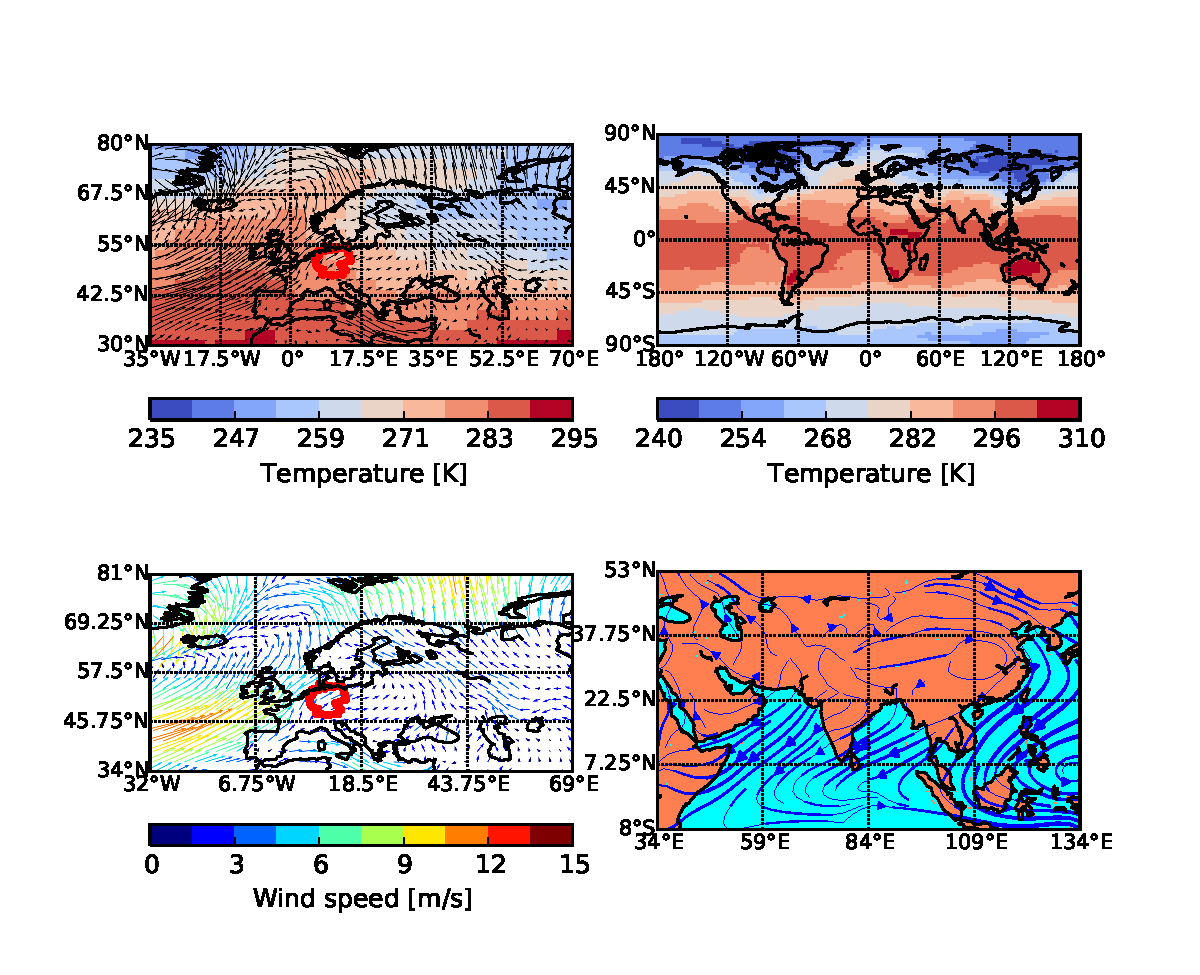
\includegraphics[width=0.9\textwidth]{figures/demo-plot-types.pdf}
	\caption{Demonstration of the different plot types with Pythons nc2map package}
	\label{fig:demo}
\end{figure}
This chapter is an introduction to the \gls{nc2map} Python module. The first section (\autoref{sec:modstruct}) deals with the general module structure, the second is a quick start showing how you can create your own maps (\autoref{sec:basic_init}) and the third is a more detailed description of the possibilities (\autoref{sec:init}).

Please also find demo scripts in the \lstinline|demo| directory of your \gls{nc2map} source files.

\section{A note about the module structure} \label{sec:modstruct}
As comparable with \lstinline|matplotlib|s axes (subplot) - figure structure, \gls{nc2map} consists of a basic class responsible for the plot (subclasses of \gls{MapBase}) and a coordinating class: \gls{MapsManager}. Each \gls{MapBase} instance thereby controls exactly one axes. A \gls{MapsManager} instance on the other hand controls multiple \gls{MapBase} instances. 

The most important \gls{MapsManager} subclass is the \gls{Maps} class which is not only designed to control many \gls{MapBase} instances but also colorbars, evaluations, output and updates to make everything interactive. Hence, the thing you probably will deal most with are instances of the \gls{Maps} class.

Furthermore, you will probably not deal with the \gls{MapBase} class, but rather with its subclasses. Those are \gls{FieldPlot}, to plot a two dimensional scalar field (e.g. temperature, see the upper row in figure \ref{fig:demo}) and \gls{WindPlot}, to visualize flows (e.g. wind or ocean currents, see the lower row in figure \ref{fig:demo}).

\section{Quick start} \label{sec:basic_init}
The simplest way how to plot open a NetCDF file and visualize it is with the \gls{Maps} class. If \lstinline|ncfile| is the variable containing the path to your NetCDF file, you can visualize the variables with
\begin{lstlisting}[label={lst:basic_init}, caption={Basic initialization of a \gls*{Maps} instance}]
	import nc2map
	ncfile = 'my-own-netcdf-file.nc'
	mymaps = nc2map.Maps(ncfile)     # initialize Maps instance
	mymaps.show()                    # show all figures
\end{lstlisting}
Or select specific variables via their name in the NetCDF file, e.g.
\begin{lstlisting}
	mymaps = nc2map.Maps(ncfile, vlst=['t2m', 'u'])
\end{lstlisting}
To visualize wind vectors, you can use the \lstinline|u| and \lstinline|v| keywords, e.g.
\begin{lstlisting}
	mymaps = nc2map.Maps(ncfile, u='u', v='v')
\end{lstlisting}
or if want to visualize only vector data without an underlying scalar field (e.g. temperature), you can do this by
\begin{lstlisting}
	mymaps = nc2map.Maps(ncfile, u='u', v='v', windonly=True)
\end{lstlisting}
You can then use the \gls{Maps.update} method to update the plot via formatoptions (see next \autoref{ch:fmt}). For example we can update the title of all plots via
\begin{lstlisting}
	mymaps.update(title='My test title of variable %(var)s.')
\end{lstlisting}
Here \lstinline|%(var)s| is replaced by the name of the specific variable that is shown in each plot, as it is used in the NetCDF file (actually you can use any meta data from the variables in the NetCDF file, see \autoref{sec:labels}). You can also update only specific \gls{MapBase} instances by using any of the meta attributes (e.g. \gls{time}, or \gls{level}, or \gls{var}) or directly via the instance specific attribute \gls{name}.

Hence let's say we only want to update the temperature (stored in variable \lstinline|t2m|) and zonal wind (stored in variable \lstinline|u|). Then we can update these \gls{MapBase} instances via
\begin{lstlisting}
	mymaps.update(title='My test title of variable %(var)s.', 
	              vlst=['t2m', 'u'])
\end{lstlisting}
For a detailed usage of the \gls{Maps.update} method please refer to the python built-in \lstinline|help| function.

Another possibility (see also next \autoref{sec:init}) would be to include the \glspl{fmt} directly in the initialization by the use of the \glssymbol{fmt} keyword via a dictionary
\begin{lstlisting}
	import nc2map
	ncfile = 'my-own-netcdf-file.nc'
	fmt = {'title': 'My test title of variable %(var)s.'}
	mymaps = nc2map.Maps(ncfile, fmt=fmt)  # initialize Maps instance
	mymaps.show()                 	       # show all figures
\end{lstlisting}
There are some demo scripts in the demo directory of your nc2map distribution which may show you some possible applications.

\section{Initializing a \texttt{nc2map.Maps} instance} \label{sec:init}
\subsection{How to specify the NetCDF files} \label{sec:init_nc}
\gls{nc2map} is primarily designed to plot NetCDF files, however it might be extended in the future (e.g. for GeoTiff files). You can simply pass in one single NetCDF file, use wildcards (e.g. $^*$ or ?) or a list of NetCDF files.
\begin{description}
	\item[One single file:] Simply use the file name, e.g. 
		\begin{lstlisting}
			mymaps = nc2map.Maps('my-netcdf-file.nc')|
		\end{lstlisting}
	\item[Using wild cards:] Same as with a single file name, e.g. 
		\begin{lstlisting}
			mymaps = nc2map.Maps('my-*-file.nc')
		\end{lstlisting}
	\item[Using multiple files:] Simply use a list of file names, e.g. 
	\begin{lstlisting}
		mymaps = nc2map.Maps(['my-netcdf-file1.nc', 'my-netcdf-file2.nc'])
	\end{lstlisting}
\end{description}
By default, \glssymbol{Maps} uses the \lstinline|netCDF4.Dataset| to visualize a single NetCDF file and the \lstinline|netCDF4.MFDataset| to visualize multiple NetCDF files. You can set manually which of the above classes is used via the \lstinline|mode| key word (\glslink{NCReader}{\lstinline|mode='NCReader'|} of \glslink{MFNCReader}{\lstinline|mode='MFNCReader|}) in the initialization of a \gls{Maps} instance. \\
Furthermore, instead of passing in the NetCDF file (or a list of NetCDF files), you can initialize the \gls{Maps} instance via setting the \lstinline|ncfile| equal to a dictionary, e.g.
\begin{lstlisting}
	mymaps = nc2map.Maps({'filename': 'my-netcdf-file.nc', 'mode': 'a'})
\end{lstlisting}
to open the NetCDF file in an editor mode. The key-value pairs of the dictionary are then assumed to represent the keyword arguments used for the initialization of the \glssymbol{ArrayReader} instance. \\
Finally you can also set the \lstinline|ncfile| keyword with an already existing \gls{reader} instance.


\subsection{Specifying what to plot via \glspl*{dimsidentifier}} \label{sec:init_dims}
The \gls{Maps} class takes a bunch of possible keywords for the initialization (see \lstinline|help(nc2map.Maps.__init__)| method for details). We already saw in listing \ref{lst:basic_init}, how to generally visualize a NetCDF file. However those commands would show all variables at the first time step, level, etc., which is maybe not desired. Therefore we can use the dimensions in the NetCDF file to be more specific. Which dimensions there are, depends on your specific NetCDF file. During the initialization of a \gls{Maps} instance, you can set any dimension you want, e.g.
\begin{lstlisting}
	# variables 't2m' and 'u' at the 2nd time step for 1st and 2nd level
	mymaps = nc2map.Maps(ncfile, vlst=['t2m', 'u'], time=1, level=[0, 1])
\end{lstlisting}
This will open 4 maps in total and assign automatically generated names \lstinline|mapo0, mapo1, mapo2| and \lstinline|mapo3| to the generated \gls{MapBase} instances. Note that for any dimension you specify in this way that is iterable\footnote{iterables in python are everything that does not raise an Error when using the built-in \lstinline|iter| function. The most prominent example are \lstinline|list|s (e.g. \lstinline|[1, 2, 3]|, or \lstinline|range(5)| or \lstinline|xrange(5)|).}, one \gls{MapBase} instance is created. Hence,
\begin{lstlisting}
	mymaps = nc2map.Maps(ncfile, vlst=['t2m', 'u'], time=range(5), level=[0, 1])
\end{lstlisting}
would create 20 maps in total (not recommended because far too much!).

Therefore, you can be more specific, by using the \glspl{name} keyword in the initialization of the \gls{Maps} instance and a dictionary. This might look like
\begin{lstlisting}
	names = {'mymap1': {'time': 1},
	         'mymap2': {'time': 1, 'level': 1}}
    mymaps = nc2map.Maps(ncfile, names=names)
\end{lstlisting}
and opens exactly two maps, one with \gls{time}\lstinline|=1| and \gls{level}\lstinline|=0| and one with \gls{time}\lstinline|=1| and \gls{level}\lstinline|=1|. This may also be useful if your variables in the NetCDF file have different dimensions.

If you do not use the \glspl{name} keyword as a dictionary but instead give another iterable (or a string with \lstinline|'{0}'| in it, e.g. \lstinline|mymodel{0}|), those will be used as names for the \gls{MapBase} instances, where the \lstinline|'{0}'| will be replaced by a counter. However, maybe it is not so useful to define your own names, but rather to give some meta attributes directly to the \gls{MapBase} via the \lstinline|meta| key. As an example
\begin{lstlisting}[label={lst:own_meta}, caption={Assigning your own meta informations}]
	mymaps = nc2map.Maps(ncfile, meta={'model': 'my first model'})
	mymaps.addmap(ncfile, meta={'model': 'my second model'})
\end{lstlisting}
will allow you to later address the \gls{MapBase} instances you want via the \lstinline|model| key, e.g.
\begin{lstlisting}
	model_maps1 = mymaps.get_maps(model='my first model')
	model_maps2 = mymaps.get_maps(model='my second model')
\end{lstlisting}
Instead of setting \lstinline|time| to 1, you can also use the time information in the NetCDF file (see \autoref{sec:time})

Those dimensions can also be changed via the \lstinline|Maps.update| method. For example
\begin{lstlisting}
	mymaps.update(fmt={'time': 1}, time=0)
\end{lstlisting}
will update all maps that currently show the first time step to the second. For time however, you can also use the \gls{Maps.nextt} and \gls{Maps.prevt} methods.

The function that is used in the initialization to add new maps to the \gls{Maps} instance, is the \gls{MapsManager.addmap} method. Hence, to add another map to the \gls{Maps} instance, you can simply use
\begin{lstlisting}
    mymaps.addmap(ncfile, ...)
\end{lstlisting}
Furthermore there is the possibility to make one dimensional line plots with data from the NetCDF file. The syntax is somewhat similar, e.g.:
\begin{lstlisting}
	mymaps = nc2map.Maps(ncfile, vlst=['t2m', 'u'], level=[0, 1], lat=0, lon=0, linesonly=True)
\end{lstlisting}
will draw lines over all time steps in the NetCDF file into one subplot for the first and second level. The corresponding method that is used is the \gls{MapsManager.addline} method.

\subsection{Specifying how to plot via \gls*{fmt} keywords}
There exist over 60 formatoptions, that can be used to exactly control the appearance of your plot. Each formatoption can be set with one single keyword (see next \autoref{ch:fmt}).

As stated already in \autoref{sec:basic_init}, you can give \glspl{fmt} directly to the initialization of the \gls{Maps} instance without using the \gls{Maps.update} method. These can be done via simply setting up a dictionary with \gls{fmt} keywords like
\begin{lstlisting}
	fmt = {'title': 'my test title',
	       'cmap': 'RdBu'}
\end{lstlisting}
However this would set the title for all variables, all time steps and all levels, in other words for all \gls{MapBase} instances that are controlled by the \gls{Maps} instance. But sometimes we do not want the same formatoptions for each \gls{MapBase} instance. For example we maybe want a colormap going from red to blue for precipitation (e.g. \lstinline|pyplots| \lstinline|'RdBu_r'| colormap) and a colormap going from blue to red for temperature (e.g. \lstinline|pyplots| \lstinline|'RdBu_r'| colormap). Therefore we can set up the \glspl{fmt} dictionary more specifically. In our case for example let's assume that precipitation is stored in the variable \lstinline|precip| and temperature in the variable \lstinline|t2m|. Our \gls{fmt} dictionary for the initialization will then be
\begin{lstlisting}
	fmt = {'title': ' %(long_name)s',
	       't2m': {'cmap': 'RdBu_r'},
	       'precip': {'cmap': 'RdBu'}
	      }
\end{lstlisting}
i.e. we used the variable identifier as a key in the \glssymbol{fmt} dictionary whose value is another \glssymbol{fmt} dictionary. Please note that the \lstinline|'title'| \gls{fmt} is set outside of the variable specific dictionaries which means that this is used as a default value for all \gls{MapBase} instances in the \gls{Maps} instance. However, since we refer here to the \lstinline|long_name| attribute inside the NetCDF file, the titles will not be the same. Hence setting up the above dictionary like
\begin{lstlisting}
	fmt = {'title': 'my test title',
	       't2m': {'cmap': 'RdBu_r',
	               'title': 'Another title'},
	       'precip': {'cmap': 'RdBu'}
	      }
\end{lstlisting}
would result in a title being \enquote{Another title} for all \lstinline|t2m| \gls{MapBase} instances and \enquote{my test title} for all the others (e.g. \lstinline|precip|).

This syntax does not only work for variables but also slightly modified for \glspl{time}, \glspl{level} and \glspl{name}. The \gls{time} step furthermore has to come with a leading \lstinline|t| followed by the time step as string, whereas the \gls{level} has to come with a leading \lstinline|l| followed by the vertical step as string. Hence
\begin{lstlisting}
	fmt = {'t0': {'title': 'This applies only for the 0-th time step'}}
\end{lstlisting}
will only modify the titles of \gls{MapBase} instances with \gls{time}\lstinline| == 0| and
\begin{lstlisting}
	fmt = {'l0': {'title': 'This applies only for the 0-th level'}}
\end{lstlisting}
will only modify the titles of \gls{MapBase} instances with \gls{level}\lstinline| == 0|.
Finally 
\begin{lstlisting}
	fmt = {'mapo0': {'title': 'This applies only for the 0-th level'}}
\end{lstlisting}
will only modify the title of the \gls{MapBase} instance with the name \lstinline|mapo0|.

Furthermore the dictionaries can be nested, where the order of hierarchy is 
\begin{equation*}
\text{\gls{name}} \succ \text{\gls{var}} \succ \text{\gls{time}} \succ \text{\gls{level}}. 
\end{equation*}
As an example look into listing \ref{lst:nested_fmt}.
\begin{lstlisting}[label={lst:nested_fmt}, caption={Example of how to define a nested formatoptions dictionary.},float,floatplacement=H]
	default_title = 'Default title'
	mapo0_title = 'Title used for mapo0'
	t2m_title = 'Default title for t2m variable'
	t2m_t2_title = 'Title for third time step of t2m variable'
	t1_title = 'Default title for second time step'

	fmt = {'title': default_title,
	       'mapo0': {'title': mapo0_title},
	       't2m': {'title': t2m_title,
	               't2': {'title': t2m_t2_title}},
	       't1': {'title': t1_title}
	       }
\end{lstlisting}
Here we set the title for the \gls{MapBase} instance with \gls{name} \lstinline|== mapo0| to \lstinline|mapo0_title|, the title for all \gls{MapBase} instances with \gls{time} \lstinline|== 1| and \gls{var} \lstinline|!= 't2m'| to \lstinline|t1_title|, the title for all time step and levels with \gls{var} \lstinline|== 't2m'| and \gls{time} \lstinline|!= 2| to \lstinline|t2m_title| and finally for \gls{var} \lstinline|== 't2m'| and \gls{time} \lstinline|== 2| to \lstinline|t2m_t2_title|.


\section{Output methods} \label{sec:output}
There are several methods of the \gls{Maps} class to save what you created:
\begin{description}
	\item[\glslink{Maps.output}{\texttt{output}}:] Save all (or some) figures into one (or more) \lstinline|pdf| files, \lstinline|png|s, \lstinline|jpg|s, etc.
	\item[\glslink{Maps.make_movie}{\texttt{make\_movie}}:] Make a movie (e.g. \lstinline|.gif| or \lstinline|.mp4|) of your \gls{MapBase} instances.
	\item[\glslink{Maps.save}{\texttt{save}}:] Creates a python script that initializes the \gls{Maps} instance in its current state (including all\gls{MapBase} and \gls{LinePlot} instances and their \glspl{fmt}.) This file can then be loaded by the \gls{nc2map.load} function to restore the \gls{Maps} instance.
\end{description}


\section{Helper functions accessing the documentation} \label{sec:helper}
There are several helper functions to cope with the visualization of your data:
\begin{description}
	\item[\glslink{show_colormaps}{\texttt{show\_colormaps}}:] This function can be used to show all the colormaps that are predefined by the \gls{nc2map} module and \lstinline|pyplot|. You can also use it to visualize your own created colormap to see, how it will finally look like.
	\item[\glslink{show_fmtkeys}{\texttt{show\_fmtkeys}:}] This function shows the possible \gls{fmt} keywords or checks whether the the keywords specified by the user are possible.
	\item[\glslink{show_fmtdocs}{\texttt{show\_fmtdocs}:}] This function shows the possible \gls{fmt} keywords or checks whether the the keywords specified by the user are possible, plus their documentation.
	\item[\glslink{get_fmtkeys}{\texttt{get\_fmtkeys}:}] This function returns a list of possible \gls{fmt} keywords as strings, or checks whether the the keywords specified by the user are possible.
	\item[\glslink{get_fmtdocs}{\texttt{get\_fmtdocs}:}] This function returns a dictionary with the possible \gls{fmt} keywords as keys and their documentation as value.
	\item[\glslink{nc2map.get_fnames}{\texttt{get\_fnames}}:] Shows the possible field names in the default shape file for the \hyperref[item:lineshapes]{\lstinline|lineshapes|} keyword (you can also use other shape files, see the corresponding function in the \gls{shp_utils} function).
	\item[\glslink{nc2map.get_unique_vals}{\texttt{get\_unique\_vals}}:] Shows the values in the default shape file for the \hyperref[item:lineshapes]{\lstinline|lineshapes|} keyword (you can also use other shape files, see the corresponding function in the \gls{shp_utils} function).
\end{description}

\section{Automatical labelling} \label{sec:labels}
One very useful feature of the \gls{nc2map} module is that you can very easily implement the meta data information of the NetCDF file in your plot. There are some labels (e.g. \hyperref[item:clabel]{clabel}, \hyperref[item:title]{title}, \hyperref[item:text]{text}, etc., see table \ref{tab:fmt_keys}) which you can set with strings that are then displayed on the plot. The following subsections describe how to use the text-like meta information of the NetCDF file in your labels (\autoref{sec:labels_text}) and how to display the time information (\autoref{sec:labels_time}).

\subsection{Using text meta data} \label{sec:labels_text}
For example let's take the variable \lstinline|t2m|. Of course you could simply set \hyperref[item:title]{\lstinline|title|}\lstinline|='Plot of t2m'| but why should you double your work if that variable is stored in the NetCDF file anyway? Therefore a much easier solution is setting \hyperref[item:title]{\lstinline|title|}\lstinline|='Plot of %(var)s'|. In fact in all labels you can replace any meta information stored (e.g. \lstinline|long_name|) by \lstinline| %(long_name)s|.

Common meta data keys are:
\begin{description}
	\item[\glslink{var}{\texttt{var}}:] Name of the variable as stored in the NetCDF file (e.g. \lstinline|t2m|)\footnote{\label{foot:MapBasedims}This information is always stored in the \gls{MapBase} instance, it is not a meta data information in the NetCDF file}
	\item[\texttt{standard\_name}:] Standard name of the variable (e.g. \lstinline|evapotranspiration| for variable \lstinline|evspsbl|)
	\item[\texttt{long\_name}:] Long name of the variable (e.g. \lstinline|Temperature|)
	\item[\texttt{units}:] Unit of the variable (e.g. \lstinline|deg C|)
	\item[\glslink{time}{\texttt{time}}:] Time step
	\item[\glslink{level}{\texttt{level}}:] Number of the vertical level
	\item[\glslink{name}{\texttt{name}}:] Name of the \gls{MapBase} instance$^\text{\ref{foot:MapBasedims}}$
\end{description}
Anyway, which meta data key is stored in a NetCDF file is determined by the NetCDF file (i.e. by the conscientiousness of the creator of the file). You can access the meta data keys via the \gls{MapBase.meta} property of the specific \gls{MapBase} instance. E.g. if you want to see the meta information of the variable \lstinline|t2m|, simply use
\begin{lstlisting}
	mymaps = nc2map.Maps('my-own-netcdf-file.nc', vlst='t2m')
	print mymaps.get_maps(vlst='t2m')[0].meta
\end{lstlisting}
Another possibility is to use the \gls{MapsManager.get_label_dict} method of the \gls{Maps} instance via
\begin{lstlisting}
	mymaps = nc2map.Maps('my-own-netcdf-file.nc', vlst='t2m')
	print mymaps.get_label_dict(*mymaps.get_maps(vlst='t2m'))
\end{lstlisting}
or the \gls{MapsManager.meta} property.

\subsection{Displaying the time} \label{sec:labels_time}
As we saw in the previous \autoref{sec:labels_text}, one possibilty to display the time step is via \lstinline| %(|\gls{time}\lstinline|)s| in our labels. However, one of the great advantages of NetCDF files is that they (almost always) follow the CF-conventions\footnote{\url{http://cfconventions.org/}} and store the time data in relative time units (e.g. \lstinline|days since 1992-10-8 15:15:42.5 -6:00|) or at least in absolute time units (\lstinline|day as %Y%m%d.%f|). \gls{nc2map} interpretes those two units and uses the python \lstinline|datetime| module to display the information in the labels. Hence to display the time of your \gls{MapBase} instance, you can use all format strings suitable with the \lstinline|strftime| function of the \lstinline|datetime.datetime| module\footnote{For a list of format strings see \href{https://docs.python.org/2/library/datetime.html\#strftime-and-strptime-behavior}{\nolinkurl{https://docs.python.org/2/library/datetime.html}}}. For example lets assume that my \gls{MapBase} instance shows the variable \lstinline|t2m| on the 2$^\text{nd}$ of March, 2015. Then setting my title as \hyperref[item:title]{\lstinline|title|}\lstinline|=' %(var)s in %B, %Y'| would result in the title \lstinline|'t2m in March, 2015'| (or {\footnotesize \texttt{'t2m in M\"arz, 2015'}} if you are in Germany).
